%!TEX root = ../../main.tex


\begin{figure}[p]
\centering
\makebox[\textwidth][c]{%
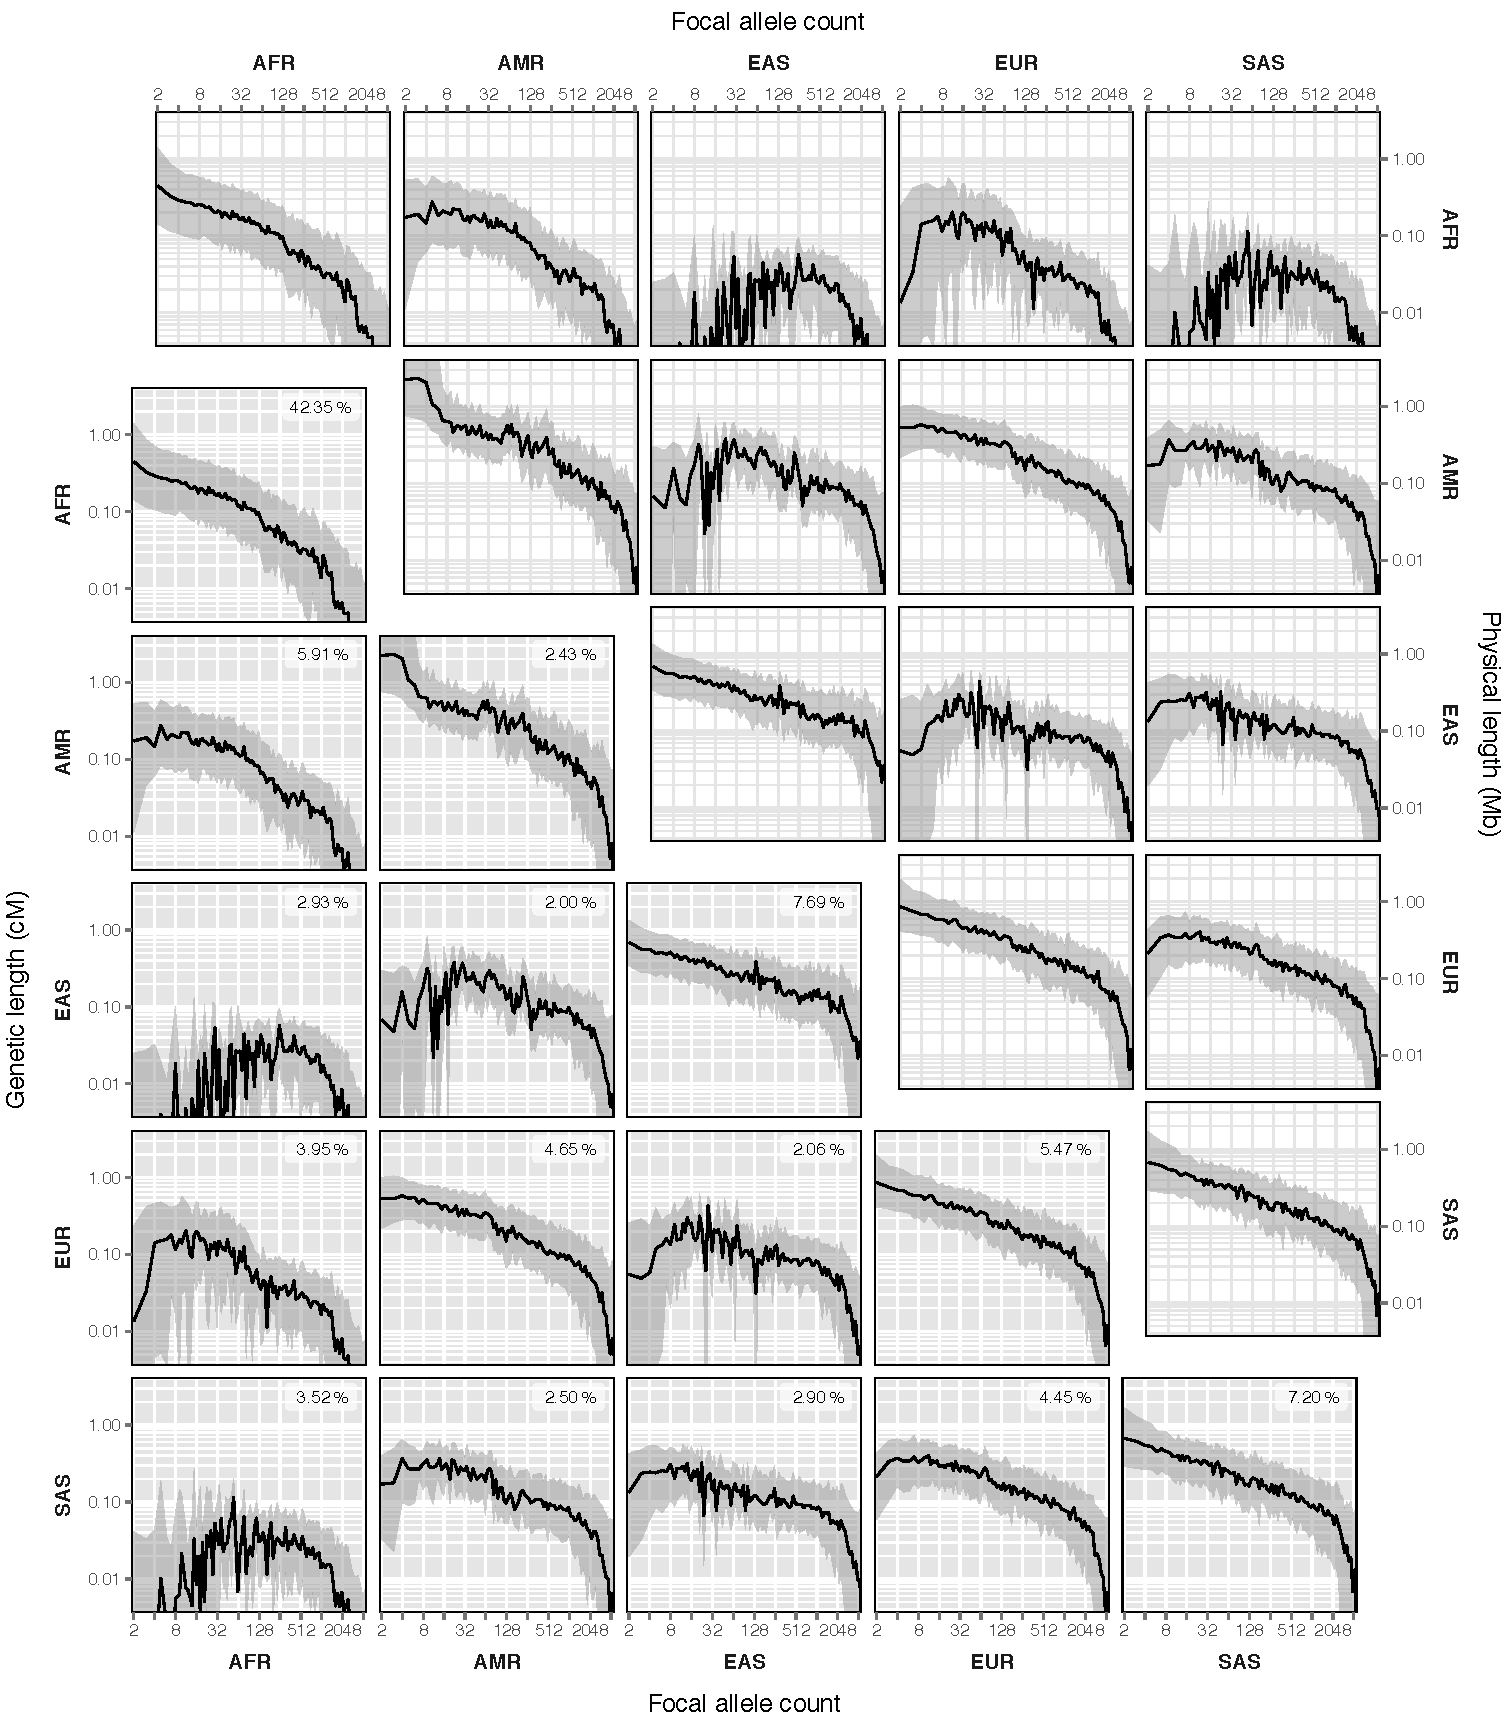
\includegraphics[width=1.1\textwidth]{./img/ch5/1KG20_pop_len_hhmm}%
}
\Caption{Shared haplotype length by population in 1000 Genomes, chromosome~20}%
{Median physical and genetic lengths are shown for haplotype pairs where individuals share a focal allele within the same or between different populations.
Note that the condition of seeing an allele shared between individuals implied that only concordant pairs were considered.
Physical lengths are given in the upper triangle (\emph{white} panels) and genetic lengths in the lower triangle (\emph{grey} panels).
The median (\emph{black} lines) is drawn between the \nth{1} and \nth{3} quartiles, where lengths were binned by focal allele count (log-scale).
The lower triangle also shown the proportions of pairs at which the focal allele was shared within or between populations.}%
{fig:1KG20_pop_len_hhmm}
\end{figure}
